\chapter{Realisierung der serverseitigen Implementierung}
\label{cha:server-impl}
In diesem Kapitel wird näher auf die Implementierung des in Kapitel \ref{sec:programmarchitektur} besprochenen Webservices eingegangen. Es enthält eine Übersicht über die genutzten Komponenten und die konkreten Techniken, welche für die Implementierung genutzt wurden. Anschließend wird gesondert auf Sicherheitsaspekte in Verbindung mit \ac{REST}ful-Architekturen eingegangen. Der hier beschriebene Web Service kann über die \ac{URL} \href{http://fit-bachelor.azurewebsites.net/}{http://fit-bachelor.azurewebsites.net/} erreicht werden. 
\section{Was ist ein Webservice?}
\label{sec:definition-webservice}
Um verteilte Systeme aufzubauen ist es nötig, eine Struktur zu implementieren, mit der Maschinen untereinander kommunizieren können. Diese Aufgabe übernehmen Webservices. Sie stellen innerhalb eines Netzwerkes Schnittstellen bereit, damit Maschinen plattformübergreifend Daten austauschen können. Hierbei wird meistens \ac{HTTP} als Träger-Protokoll genutzt, um eine einfache Interoperabilität zu gewährleisten.\footcite{Definition-Webservice} Die dabei angeforderten Daten werden in der Regel im \textit{\ac{XML}}- oder \textit{\ac{JSON}}-Format übermittelt. 
\subsection{Besonderheiten eines RESTful Webservices}
\label{sec:definition-rest}
Da Webservices in der Regel \ac{HTTP} als Protokoll verwenden, wurde die Idee zur Implementierung eines Webservices erweitert, um die Möglichkeiten des Protokolls besser zu benutzen. Daraus entstand das Programmierparadigma \ac{REST}. Mit einem \ac{REST}-Server bzw. einem \ac{REST}ful Webservice bezeichnet man einen Webservices, welcher die strikte Nutzung von \ac{HTTP} als Programmierparadigma umsetzt.  Dies meint, dass sich, wie im Internet üblich, \ac{URI} zur eindeutigen Identifikation von Ressource genutzt werden. Nachfolgend werden einige Prinzipien von \ac{REST} näher beleuchtet.

\subsubsection*{Adressierbarkeit}
Im Gegensatz zu anderen Webservice-Implementierungen stellen \ac{REST}ful Webservices keine Methoden oder aufrufbare Funktionalitäten zu Verfügung, sondern ausschließlich Ressourcen. Dies hat den Vorteil, dass die Schnittstelle leicht und eindeutig beschrieben werden kann, da ein Aufruf einer \ac{URL} an den \ac{REST}-Service immer eindeutig auf eine Ressource zeigt, ohne das Abhängigkeiten oder ein Kontext berücksichtigt werden müssen. \\
In den meisten Fällen, wie auch in den Anwendungsfällen dieser Arbeit, soll der Webservice \textit{\ac{CRUD}}-Funktionalitäten bereitstellen. Damit die Schnittstelle nicht durch unnötig viele unterschiedliche \ac{URL}s aufgebläht wird, sieht der \ac{REST}ful-Ansatz die Verwendung der verschiedenen \ac{HTTP}-Verben vor, um mit den Ressourcen zu Interagieren. Dazu werden zwei Arten von \ac{URL}s unterschieden, um in Kombination mit \ac{HTTP}-Verben verschiedene Aufgaben zu erfüllen. Zur Veranschaulichung sollen uns folgende zwei \ac{URL}s dienen:
\begin{itemize}
\item http://myRestService.de/Schedule
\item http://myRestService.de/Schedule/123
\end{itemize}
Es fällt auf, dass die beiden \ac{URL}s sich bis auf das letzte Segment gleichen. Im ersten Fall wird die \ac{URI} als \textit{Collection \ac{URI}} bezeichnet, da hiermit die Gesamtheit aller Trainingspläne angesprochen wird. Im zweiten Fall wird die ID einer Trainingsplans benutzt und mit einer konkreten Trainingsplan-Ressource zu interagieren. Man spricht hier von einer \textit{Element \ac{URI}}.\footcite[S. 12ff.]{Building-a-REST-Service} Diese können mit verschiedenen \ac{HTTP}-Verben kombiniert werden.\footcite[S. 26ff.]{REST-und-HTTP}
\subsubsection*{Nutzung von HTTP-Verben}
Um den Rahmen der Arbeit nicht zu überspannen, wird sich hier nur auf die Vorstellung der vier meist verwendeten \ac{HTTP}-Verben beschränkt:\\
Das Verb GET ruft eine Ressource vom Server ab, wobei diese nicht verändert wird. Bei Nutzung einer \textit{Collection \ac{URI}}, werden alle Einträge dieser Entität als Verbundstruktur abgerufen. Jedes Element der Struktur beinhaltet die \textit{Element URI} auf das konkrete Element. Wird GET auf eine \textit{Element URI} aufgerufen, wird das konkrete Objekt aufgerufen. Hierbei antwortet der Server, dem \ac{HTTP}-Standard folgend, mit dem Status-Code \textit{200 (OK)} bei erfolgreicher Suche oder \textit{404 (Not Found)}, wenn keine Ressource gefunden wurde.\\
Das POST wird zur Erstellung neuer Inhalte verwendet. Bei Nutzung von \textit{Element \ac{URI}s} wird versucht, die ID für das neue Element zu benutzten. In der Regel wird das ID Management aber auf dem Server implementiert, sodass eine Collection \ac{URI} zur Erstellung von Elementen zum Einsatz kommt.\\
Mit dem HTTP-Verb PUT wird eine vorhandene Ressource geändert oder hinzugefügt. Obwohl es \ac{REST}-conform wäre, eine Collection \ac{URI} per PUT aufzurufen, wird dies selten implementiert, da der normale Anwendungsfall ist, dass ein einzelnes Objekt geändert werden soll. Stattdessen wird sich auf \textit{Element \ac{URI}s} beschränkt. Ist eine Ressource mit der übergebenen ID nicht vorhanden, wird je nach Implementierung entweder ein neues Objekt mit der ID erstellt (\textit{Statuscode 201 (Created)}) oder die Verarbeitung verweigert. Der Server gibt dann den Statuscode \textit{400 (Bad Request)} oder \textit{404 (Not Found)}  zurück. \\
Das letzte HTTP-Verb, welches an dieser Stelle vorgestellt werden soll, ist DELETE. Wie der Name vermuten lässt, wird damit eine Ressource vom Server entfernt. Wie auch bei PUT wird in der Regel auf eine Implementierung von DELETE als \textit{Collection \ac{URI}} verzichtet, da sonst alle Einträge einer Entität gelöscht werden können. Im Erfolgsfall wird mit dem Statuscode \textit{200 (Ok)} geantwortet und bei Fehlern mit \textit{400 (Bad Request)} oder \textit{404 (Not Found)}.\footcite[S. 26ff.]{REST-und-HTTP}
\subsubsection*{Zustandslosigkeit}
Da das statuslose Protokoll \ac{HTTP} zum Datenaustausch genutzt wird, ist ein \ac{REST}ful Webservice so zu implementieren, dass alle Informationen, welche für die Kommunikation notwendig sind, bei jeder Anfrage mitgesendet werden. Was vordergründig als Nachteil erscheint, ist ein wesentlicher Vorteil. Dadurch, dass jeder Request alle nötigen Informationen mitliefert, ist es nicht nötig, Kontext der Kommunikation über mehrere Requests auf dem Server zu verwalten. Dadurch kann ein \ac{REST}ful Webservice sehr leicht skaliert werden.\footcite[S. 26ff.]{REST-und-HTTP}
\subsubsection*{Daten sind unabhängig von der Präsentation}
Das \ac{REST}ful-Paradigma besagt, dass Daten losgelöst von einer Repräsentation bereit gestellt werden. Darum ist ein \ac{REST}ful Webservice so zu implementieren, dass der Client das gewünschte Datenformat anfragen kann. Bei Nutzung des Protokolls HTTP wird dies in der Regel über die Header-Eigenschaft \textit{accept} realisiert, welche gewünschten Datenformate angibt. Wird dieses nicht vom Server unterstützt, werden die angeforderten Daten in einem Standard-Format zurückgegeben. \footcite[S. 26ff.]{REST-und-HTTP}
\section{Aufbau der Komponenten}
\label{sec:aufbau-Komponenten}
In diesem Kapitel wird beschrieben, wie der zuvor theoretisch beschriebene \ac{REST}-Ansatz für das Projekt umgesetzt wurde. Der Server besteht aus zwei Teilen: Der Datenbank und der Web \ac{API}, welche jeweils gesondert vorgestellt werden. \\
Die Web \ac{API} bietet eine Schnittstelle zum Abrufen der Daten mittels \ac{HTTP}. Diese wurde nach dem Design-Pattern \textit{\ac{MVVM}} aufgebaut. Die erzeugten Objekte, welche Tupel einer Datenbank-Relation darstellen, werden aus speziell dafür präparierten Model-Klassen erzeugt. Bevor diese Daten dann über die Web \ac{API} bereitgestellt werden, werden sie vom Model in ein ViewModel übertragen. Hierbei wird, nach dem Grundgedanken des \gls{Seperation-of-Concerns}, klar zwischen den Models für die Datenbank und den ViewModels, welche die Web \ac{API} benutzt, unterschieden.
\subsection{Datenbank}
\label{ssec:aufbau-server-db}
Da bei der Umsetzung des Projekts konsequent auf Produkte von Microsoft gesetzt wurde, wurde als Datenbanksystem \textit{\ac{MSSQL}} gewählt. Dies hat den Vorteil, dass das \textit{\gls{MSEF}}, welches sehr gut für die Nutzung mit einer Web \ac{API} optimiert ist, als \gls{OR-Mapper} genutzt werden kann. Dieser bietet das Design-Pattern \textit{Code First}. Das bedeutet, dass anhand präparierter Model-Klassen die benötigten Relationen in der Datenbank automatisch erzeugt wird. \footcite{entity-framework-code-first}\\
An den folgenden Beispielen wird exemplarisch beschrieben, wie die Model-Klassen aufgebaut wurden und wie sich daraus die Struktur der Datenbank ergibt. Grundlage für Model-Klassen ist das Interface \textit{IEntity}(Quellcode \ref{lst:IEntity}):
\lstinputlisting[caption=Basisinterface für DB-Repräsentationen, label=lst:IEntity, style=sharpc]{content/listings/IEntity.cs}
Das Interface gewährleistet, dass jede Datenbank-Entität einen eindeutigen Schlüssel besitzt.
Eine konkrete Implementierung für eine Model-Klasse sieht man im Quellcode-Beispiel \ref{lst:Schedule}, in der die Trainingspläne implementiert sind:
\lstinputlisting[caption=Modelklasse für Trainingspläne, label=lst:Schedule, style=sharpc]{content/listings/Schedule.cs}
Hierbei zeigt sich gut, was mit einer präparierten Klasse gemeint ist. Über die Annotation \textit{Required} wird definiert, dass die Eigenschaft \textit{Name} zwingend bei Insert- und Update-Operationen gesetzt werden muss. \\
Gleichzeitig sieht man an diesem Beispiel, wie das Entity Framework über Namenskonventionen Verbindungen zwischen Entitäten auflöst. Auf Grund des Aufbaus der Klasse \textit{Schedule} wird eine einwertige Fremdschüssel-Beziehung zu der Model-Klasse \textit{User} erzeugt, da folgende Bedingungen erfüllt sind:
\begin{itemize}
\item Die Klasse \textit{User} besitzt eine Eigenschaft \textit{ID} vom Datentyp \textit{string}
\item Die Klasse \textit{Schedule} besitzt eine Eigenschaft \textit{UserID} vom Datentyp \textit{string}
\end{itemize}
Auch die Erstellung einer mehrwertigen Beziehung lässt sich aus dem Code-Beispiel \ref{lst:Schedule} ablesen: Da es eine Entität gibt, welche \textit{Exercise} heißt und die Model-Klasse \textit{Schedule} eine Verbundstruktur besitzt, welche \textit{Exercises} heißt, wird implizit eine Verbindung zwischen den Relationen in der Datenbank angelegt. \footcite{entity-framework-code-first}
\subsection{Web API}
\label{ssec:aufbau-webapi}
Die Umsetzung der \ac{REST}-Schnittstelle wurde mit Hilfe des Microsoft-Frameworks \textit{ASP.NET Web API 2} (kurz \textit{Web \ac{API}-Framework}) realisiert. Dieses ermöglicht es, Controller-Methoden zu schreiben, welche über definierte Routen per HTTP aufgerufen werden können. Hierbei wird die Umsetzung im Sinne des \ac{REST}-Paradigmas durch vorhandene Funktionen unterstützt.\footcite[S. 2ff.]{Building-a-REST-Service}\\
Dies wird beispielhaft an der Methode aus  Quellcode-Abbildung \ref{lst:ScheduleController} gezeigt:
\lstinputlisting[caption=POST-Methode zur Erstellung eines Trainingsplans, label=lst:ScheduleController, style=sharpc]{content/listings/SchedulesController.cs}
Im Beispiel fällt auf, dass das \textit{Web \ac{API}-Framework} die Nutzung von Annotationen fördert: Das Routing kann durch die Annotationen \textit{Route} (Zeile \ref{line:SchedulesController_Route}) an der Methode und \textit{RoutePrefix} (Zeile \ref{line:SchedulesController_RoutePrefix}) am gesamten Controller konfiguriert werden. Neben der Konfiguration der Route muss dem Framework noch mitgeteilt werden, welche \ac{HTTP}-Verben in dieser Methode zulässig sind. Das \textit{Web \ac{API}-Framwork} bietet hierfür pro Verb eine eigene Annotation. Im Codebeispiel \ref{lst:ScheduleController} wird über die Annotation \textit{HttpPost} (Zeile \ref{line:SchedulesController_HTTPVerb}) ausgesagt, dass nur POST-Request durch diese Methode verarbeitet werden.\footcite{webApi-AttributeRouting} \\
Das Framework versucht die empfangenen Daten in einem ViewModel-Objekt zu kapseln und anschließend zu validieren. Die dafür genutzten Validatoren werden direkt im View-Model als Annotationen angegeben.\footcite{webApi-Validation} Die Klasse \textit{EntryModel} (Beispiel \ref{lst:EntryModel}) zeigt die Möglichkeit in Zeile \ref{line:EntryModel_Annotation_1} und \ref{line:EntryModel_Annotation_2}. \\ 
\lstinputlisting[caption=Basis-Model-Klasse, label=lst:EntryModel, style=sharpc]{content/listings/EntryModel.cs}
Schlägt die Validierung fehl, werden die Fehler mit dem passenden Statuscode zurückgegeben. Andernfalls werden die Daten per \gls{Factory}-Klasse in ein Model konvertiert und per \gls{Repository}-Klasse in der Datenbank persistiert. Anschließend wird dem ViewModel, im Sinne des \ac{REST}-Gedankens, ein URL zur GET-Methode mit der ID des neu erstellten Objekts übergeben. 
\subsubsection*{Swagger}
\label{sssec:Swagger}
Da die Web \ac{API} zur Entwicklung der Clients benötigt wurde, wurde schnell die Notwendigkeit einer Dokumentation des aktuellen Stands klar. \\
Aus diesem Grund wurde \textit{Swagger} in die Web \ac{API} integriert. \textit{Swagger} ist ein quelloffenes Framework zur Dokumentation von \ac{REST}ful Web \ac{API}s, welche von vielen großen Konzernen genutzt wird\footcite{swagger}. Durch Nutzung des \gls{NuGet}-Packets \textit{Swashbuckle} konnte durch hinzufügen von Kommentaren und Annotationen eine vollständige und übersichtliche Dokumentation erstellt werden\footcite{implementing-Swagger}. \\
Da das Authorisierungsprotokoll OAuth in Version 2 (kurz: \textit{OAuth2}) zum Durchführungszeitpunkt des Projekts noch nicht von \textit{Swagger} unterstützt wird, kann das Ausführen von API-Request aus \textit{Swagger} heraus nur für Methoden durchgeführt werden, für die keine Autorisierung des Nutzers benötigt wird. \\
Die Dokumentation ist unter \href{http://fit-bachelor.azurewebsites.net/swagger}{http://fit-bachelor.azurewebsites.net/swagger} aufrufbar. 
\begin{figure}[h]
\centering
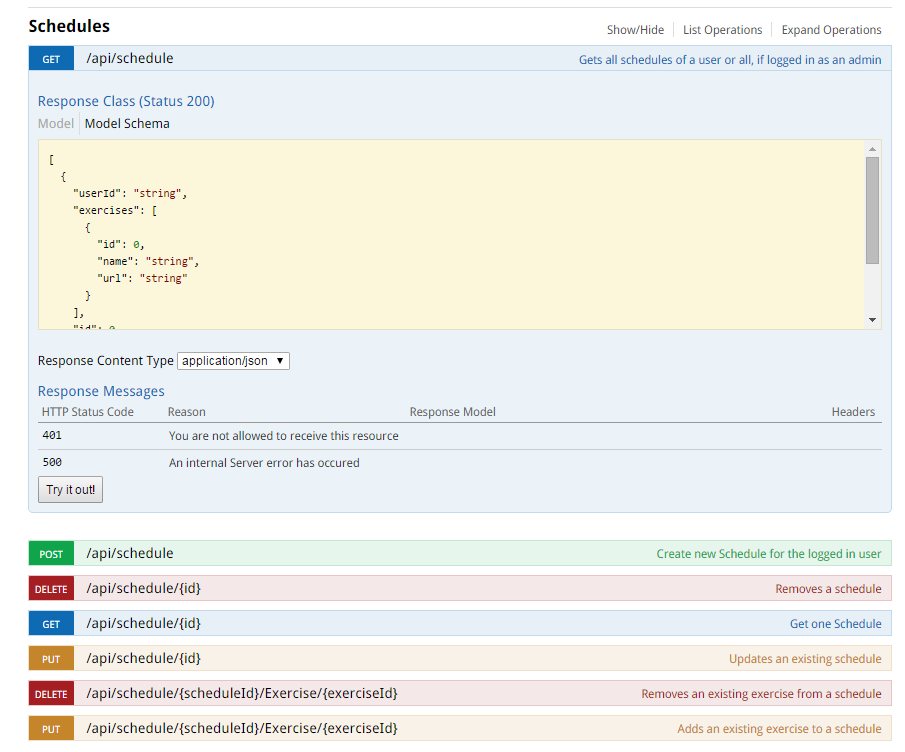
\includegraphics[width=0.8\linewidth]{content/images/Swagger-UI-fIT}
\caption{Swagger UI der Web Api}
\label{pic:swagger-UI}
\end{figure}


\section{Authentifizierung \& Autorisierung}
\label{sec:server-authorisierung}
Wie bereits in Kapitel \ref{sec:rollen-konzept} beschrieben, darf nicht jeder Nutzer auf alle Daten zugreifen. Um dies zu bewerkstelligen, wurde ein Login-Mechanismus implementiert, welcher bekannte Nutzer authentifiziert. Da jedoch nicht alle authentifizierten Nutzer alle bereitgestellten Web \ac{API}-Methoden benutzen dürfen wurden auf Basis des \ac{Role-Based Access Models} Rollen implementiert, welche den Nutzer zur Nutzung verschiedener Aufrufe autorisieren. Zur Umsetzung dieser Anforderungen wurde das Protokoll \textit{OAuth2} implementiert.\footcite{online:WebApi_Authorize}
\subsection{OAuth2}
\label{ssec:oauth2}
OAuth2 ist ein Protokoll zur Authentifikation und zur Delegation von Zugriffsrollen. Die Struktur von OAuth2 kennt vier Instanzen, welche diesem Vorgang miteinander kommunizieren, nämlich Client, Resource Owner, Authorization Owner und Resource Server.\footcite[S. 286]{book:AngularJs:Steyer2015} 
\begin{figure}[h]
\centering
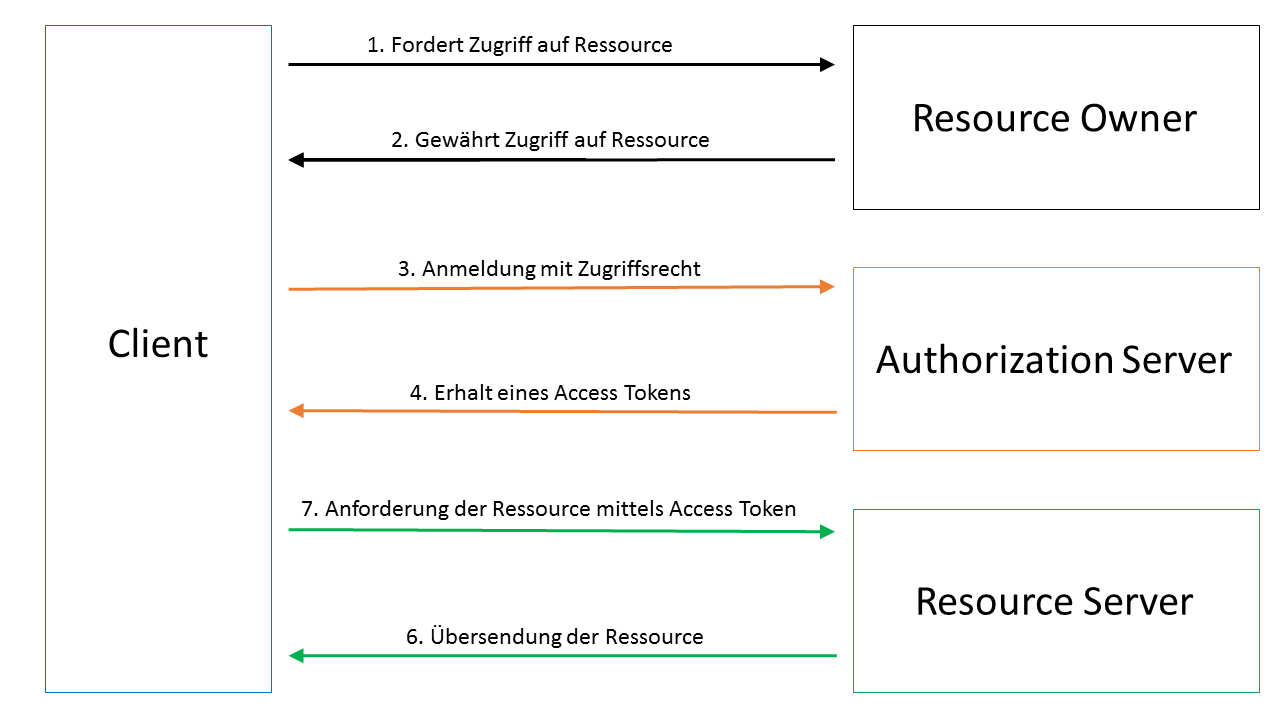
\includegraphics[width=1\linewidth]{content/images/OAuth2}
\caption{Resourcenzugriff durch OAuth2}
\label{pic:OAuth2}
\end{figure}
\subsubsection*{Client}
Der \textit{Client} ist ein Endpunkt, welcher eine Ressource (beispielsweise Trainingspläne) abrufen möchte. In unseren Fall ist das die Web- oder die native App. Diese kommunizieren jeweils mit den anderen Instanzen.
\subsubsection*{Resource Owner}
Der \textit{Resource Owner} ist, wie der Name schon sagt, der Besitzer der geforderten Ressource. Der \textit{Client} erfragt im ersten Schritt beim \textit{Resource Owner} den Zugriff zu einer Ressource.\\
Im diesem Projekt registriert sich der Nutzer an der Web \ac{API}. Anschließend kann er unter seinem Account Daten(Trainingspläne und Trainings) anlegen. Diese angelegten Daten sind die geforderten Ressourcen. Da diese vom Nutzer selbst angelegt wurden, erhält er automatisch die Erlaubnis (\ac{Grant}) zur Anfrage am \textit{Authorization Server}\footcite{online:Implemented_OAuth_WebToken}.
\subsubsection*{Authorization Server}
\label{sssec:authorization-server}
Der Nutzer meldet sich nun mit der erhaltenen Erlaubnis am \textit{Authorization Server} an. Dieser hat Kenntnis über alle vorhandenen Nutzer und deren Rollen\footcite{online:Implemented_OAuth_Roles}. Bei erfolgreicher Anmeldung erhält der Nutzer ein kurzlebiges \textit{Access-Token}, dem Typen des Access-Tokens, dessen Ablaufdatum und ein langlebiges \textit{Refresh-Token}. Das Access-Token wird im nächsten Schritt benutzt, um die gewünschte Ressource anzufordern. Das \textit{Refreh-Token} wird benutzt, um ein neues \textit{Access-Token} anzufordern. Die beiden Token-Arten werden nochmal genauer in Abschnitt \ref{ssec:jwt-bearer} besprochen.\footcite[S. 287]{book:AngularJs:Steyer2015} 
\subsubsection*{Resource Server}
Der \textit{Resource Server} enthält die geforderten Ressourcen. Ab dieser Anfrage muss das Access-Token bei jeder Anfrage mitgesendet werden. Konkret passiert dies, indem im Header der Anfrage um den Schlüssel \textit{authorization} erweitert wird.

Durch diese strikte Trennung dieser Instanzen ist es ohne weiteres möglich, dass unterschiedliche Systeme die jeweiligen Aufgaben übernehmen. Daraus hat sich in letzter Zeit etabliert, dass es immer häufiger \ac{Single-Sign-On}-Szenarien implementiert werden. Dabei muss ich der Nutzer nur an einer Stelle registrieren (z.B. Bei Facebook oder Twitter). Will der Nutzer nun auf eine andere Ressource zugreifen, kann der Ressource-Server ein Access-Token vom Facebook-Authorisierungsserver akzeptieren. Dies hat für den Nutzer den Vorteil, dass er sich nicht bei mehreren Seiten registrieren muss, sondern jedes mal Zugriff über den Authorisierungsserver mithilfe seiner Credentials erhält. \footcite[S. 294]{book:AngularJs:Steyer2015} 
\subsection{JWT and Bearer Token}
\label{ssec:jwt-bearer}
Sowohl das Access-Token als auch das Refresh-Token sind JWTs (JSON Web Tokens). Das sind codierte und meistens auch signierte Repräsentationen von Daten. Zur genaueren Betrachtung des Aufbaus, wird folgend ein Access-Token näher beschrieben. Es besteht aus 3 Teilen\footcite[S. 289]{book:AngularJs:Steyer2015}, welche jeweils als \ac{base64}-String codiert wurden und mit einem Punkt getrennt sind. Die Bestandteile sind:
\begin{itemize}
\item \textbf{Header}\\Hier wird der Typ des Tokens und der Algorithmus, welcher für die Verschlüsselung benutzt wurde, angegeben. 
\item \textbf{Payload} \\Die zu übermittelnden Daten werden als JSON-Objekt bereitgestellt. Das Objekt enthält sowohl die Informationen für die Kommunikation, wie beispielsweise den Nutzername und Rollen, als auch Meta-Daten über das Token (z.B. das Ablauf-Datum).
\item \textbf{Signatur}\\Damit gewährleistet ist, dass die Daten unverändert wurden, werden Sie mit einem Client-Secret verschlüsselt. Dies bedeutet aber auch, dass der Server jeden Client kennen muss, welcher sich beim \textit{Authorization Server} anmelden will. \\Da es sich bei diesem Projekt um einen Prototypen handelt, wurde die Implementierung der Client-Verwaltung nicht durchgeführt, da es für den Ablauf nicht zwingend benötigt wird. Der Server lässt alle gültigen Access-Token und alle bekannten Refresh-Tokens zu. Im produktiven Einsatz müsste diese Komponente dringend nachträglich implementiert werden, da sonst eine Sicherheitslücke entsteht.\footcite{online:understanding-jwt}
\end{itemize}
Wie bereits im Abschnitt zum \textit{Authorization Server} (siehe \ref{sssec:authorization-server}) beschrieben, wird für das \textit{Access-Token} eine recht kurze- und für das \textit{Refresh-Token} eine sehr lange Lebenszeit gewählt. Dies hat zwei Vorteile:\\
Das Access-Token wird bei Request an den Server mitgesendet. Sollte das Token von Dritten abgefangen werden, können diese nur für kurze Zeit im Namen des Nutzers Aktionen durchführen. Das Abgreifen eines solchen Tokens wird im produktiven Gebrauch durch zusätzliche Sicherheitsmaßnahmen, wie die Nutzung von \ac{HTTPS} erschwert. \\Da das Refresh-Token nur zum Erneuern des Access-Tokens benutzt wird, ist die Gefahr, dass es abgefangen wird wesentlich geringer, wodurch die lange Lebensdauer vertretbar ist. \\
Außerdem bleiben durch die kurze Lebensdauer des Access-Tokens die Daten immer aktuell. Sollte sich an den Daten des Nutzers etwas ändern (z.B. wird eine Rolle hinzugefügt oder entzogen) wird diese Änderungen beim nächsten Abrufen eines Access-Tokens in die Payload codiert\footcite{online:Implemented_OAuth_RefreshToken}. Somit ist immer gewährleistet, das der Nutzer nur die Funktionalität nutzt, für die er auch autorisiert ist. 
\subsection{Zugriff per CORS}
\label{ssec:cors}
Im letzten Abschnitt wurden Maßnahmen beschrieben, damit nur autorisierte Nutzer an geschützte Daten herankommen. Mit \ac{CORS} wird ein weiterer Mechanismus vorgestellt, welcher den Zugriff auf die Daten per \ac{Ajax} beschränkt. \\
Um den Nutzer davor zu schützen, dass eine Webseite im Hintergrund Daten von anderen Quellen nachläd, ist in jedem Browser eine \ac{Same-Origin-Policy} implementiert. Diese besagt, dass nur Daten aus der gleichen Domäne, aus der der AJAX-Aufruf abgesetzt wurde, abgerufen werden dürfen. \\
Da es trotzdem häufig nötig ist, auf fremden Domains zuzugreifen, wurden schnell Workarounds wie das Vorgehensmodell \ac{JSONP} eingeführt. Da diese jedoch von vielen Entwicklern als unelegant empfunden wurden\footcite[S. 102]{book:AngularJs:Steyer2015}, wurde mit CORS ein standardisierter Weg entwickelt, um Daten von fremden Domains abzurufen. Hierbei wird beim Server eine Liste an gültigen Domains für eine Cross-Domain-Anfrage hinterlegt.  \\
Soll nun vom Browser eine Anfrage an den Server gesendet werden, wird über das HTTP Verb unterschieden, ob durch diese Anfrage eine Server-Datum verändert wird. Dies geschieht bei PUT, DELETE und POST, wobei letzteres eine Ausnahme bildet. Werden per POST Daten in einem Format übermittelt, welches beim Absenden eines Formulars genutzt wird(z.B. application/x-www-form-urlencoded), wird die Anfrage wie ein nicht-ändernder Aufruf behandelt. \\
Wenn nun eine Daten-Änderung im Sinne von CORS durch den Aufruf angestoßen wurde oder wenn der Aufruf zusätzliche Schlüssel im Header enthält, wird vor der Ausführung ein \ac{Preflight} gesendet. Dies ist eine OPTIONS-Anfrage, welche genutzt wird, um die Durchführung der bevorstehenden Anfrage zu validieren.
Enthält die Antwort im Header nicht den Schlüssel \textit{Access-Control-Allow-Origin} mit der aufrufenden Domäne, wird vom Browser ein Fehler erzeugt. Andernfalls wird die Abfrage an den Server gesendet\footcite[S. 102]{book:AngularJs:Steyer2015}. Dadurch ist gewährleistet, dass nur berechtigte Clients anfragen an den Server senden. Es wurde auf weitere Implementierung von \ac{Polyfills} verzichtet, da CORS bereits in allen modernen Browsern genutzt werden kann\footcite{online:can-i-use:cors}.
\section{Testen der Funktionalität}
\label{sec:server-tests}
Die erwartete Funktionsweise des Servers ist Grundvoraussetzung für die Umsetzung der Clients. Um diese zu bewerkstelligen wurde die \textit{ManagementApi} entwickelt. Dies ist ein portable DLL, welche alle Anfragen an den Server in Methoden kapselt. Hierbei wurde bei der Erstellung der DLL darauf geachtet, dass sie sowohl in klassischen Testprojekten als auch zur Umsetzung der nativen App genutzt werden kann. Hierbei wurde darauf geachtet, dass alle Methode asynchron aufrufbar sind.
Die so erzeugten Methoden iterative entwickelt und direkt getestet. Hierbei wurden zur Verifikation der Funktionalität ausschließlich Positivtests erstellt. So war sichergestellt, dass jede Methode der \textit{ManagementApi} die gewünschten Änderungen auf dem Webservice durchführt. \\Der nachfolgende Codeausschnitt zeigt beispielhaft die Entwicklung eines Testfalls:
\lstinputlisting[caption=Implementierung des Tests 'Nutzer kann eigene Daten anpassen', label=lst:ClientTests.Users, style=sharpc]{content/listings/ClientTests.Users.cs}
Dadurch, dass sowohl der ManagementService als auch die ManagementSession das Interface \textit{IDisposable} implementieren, kann für jeden Test unabhängig eine neue Session erstellt werden, in der der Test läuft. Ist der \textit{using}-Block vollständig durchlaufen, wird die Dispose-Methode aufgerufen, welche die verwendeten Ressourcen wieder freigibt (siehe Zeile \ref{line:ClientTests:Disposable}f.). 